\chapter{Experiment}
Experimentom v našej práci je meranie hĺbky pamäte a vyhodnotenie vplyvu rôznych
hyperparametrov a typov kontextov na hĺbku pamäte rekurentných SOM.
Cieľom nášho experimentu je aj nájdenie 
optimálnej kombinácie parametrov pre všetky typy porovnávaných sietí a ich vzájomné porovnanie.

\section{Výber konkrétnych trénovacích množín pre experiment}
Trénovacie množiny sme sa snažili zvoliť
takým spôsobom aby sme na nich vedeli otestovať rôzne vlastnosti rekurentných sietí.

Pre náš experiment sme vybrali 3 trénovacie množiny.
Hlavnou trénovaciou množinou, ktorú používame v našom experimente, je náhodne generovaná 
sekvencia dlhá 1000 znakov, ktorá pozostáva z písmen $abcd$.
Táto sekvencia obsahuje dostatočné množstvo regularít a malé množstvo unikátnych znakov a teda
aj siete s relatívne malým počtom neurónov sa na nej vedia dobre natrénovať.
Používame ju pri hľadaní optimálnych parametrov pre jednotlivé typy sietí.

Ako druhú trénovaciu množinu sme zvolili sekvenciu dlhú 1000 znakov, pričom znaky sú generované
špeciálnym pravdepodobnostným stavovým automatom (Reberov automat). Automat generuje znaky z množiny znakov $ptvxse$.
Táto sekvencia je pre SOMky ťažšia na naučenie a používame ju na overenie toho, či sú siete schopné natrénovať sa aj
na zložitejších nenáhodných sekvenciách. Pri SRN je použitie tejto trénovacej množiny zaujímavejšie,
vďaka vlastnostiam, ktoré SRN má.

Tretí dataset je úryvok z korpusu anglického textu, z ktorého sú odstránené špeciálne znaky a medzery.
Keďže ide o reálny zmysluplný text, nie je to úplne náhodná postupnosť znakov, ale obsahuje určité vzory a opakovania, ktoré by siete mohli vedieť zachytiť
vo svojej vnútorenej reprezentácii.
Tento dataset používame čisto iba na overenie, či 
sú SOMky schopné zachytiť vzory aj \\ v prirodzenom jazyku a teda či sú použiteľné aj pre 
reálne dáta.

\section{Hľadanie optimálnych parametrov sietí}
Na to aby sme mohli porovnať hĺbku pamäte rôznych typov sietí museli sme najskôr
nájsť kombináciu parametrov pri ktorých daný typ siete dosahuje najnižšiu kvantizačnú chybu a 
najvyššie hodnoty pamäťových hĺbok. 

Pri trénovaní samoorganizujúcich sa máp môžeme meniť a optimalizovať veľké množstvo parametrov. 

Ako prvé sme museli správne nastaviť veľkosť okolia víťazného neurónu.
Veľkosť okolia by nemala byť počas trénovania konštantná, ale mala by sa postupne zmenšovať.
Vo fáze doľaďovania by mala byť čo najmenšia.
Excitáciu neurónu v určitom kroku trénovania určuje excitačná funkcia. Zvolili sme spojitú
excitačnú funkciu so spojitým gausovským okolím. 
\begin{equation}
    N(i^{*}, i) = \exp^{- \frac{d^{2}_{E}(i^{*}, i)}{\lambda^{2}(t)}}
\end{equation}
Najvyššiu hodnotu má excitačná funkcia pre víťazný neurón, hodnota excitačnej funkcie pre ostatné 
neuróny v sieti závisí od ich euklidovskej vzdialenosti v mriežke neurónov od ich víťaza. Veľmi vzdialené neuróny 
majú takmer nulovú excitáciu a updatujú svoje váhy minimálne.
Dôležitý je parameter $\lambda$, ktorým znižujem veľkosť okolia postupne v jednotlivých epochách.
Najlepšie výsledky (najnižšie hodnoty kvantizačnej chyby) sme dosiahli pri použití nasledujúceho vzťahu pre výpočet hodnoty tohto parametra
v jednotlivých epochách:
\begin{equation}
    \lambda{(t)} = \lambda_{i} \cdot (\lambda_{f} /\ \lambda_{i})^{t /\ t_{max}}
\end{equation}
Kde $\lambda_{f}$ je konštanta, ktorá určuje rýchlosť klesania. 
$\lambda_{i}$ je polovica maximálnej vzdialenosti dvoch neurónov v mape, resp. 
vzdialenosť dvoch neurónov na koncoch diagonály mriežky neurónov.
$t$ je číslo aktuálnej epochy trénovania. Parametrer $t_{max}$ je celkový počet 
epôch trénovania.

Ďaľšie parametre:

\begin{itemize}
    \item \textbf{Rýchlosť učenia} \\
    Rovnako ako okolie aj rýchlosť učenia siete by mala počas
procesu trénovania postupne klesať. Na začiatku chceme aby sa váhy menili čo najviac
a ku koncu učenia chceme aby sa doľadovali iba detaily.
Máme na výber 2 možnosti. Postupné znižovanie rýchlosti učenia po každom vstupe, alebo 
postupné znižovanie rýchlosti učenia po jednotlivých epochách, pričom počas každej epochy
je rýchlosť učenia konštantná. 
V naších experimentoch sme dosiahli lepšie výsledky postupním 
znižovaním rýchlosti učenia po každom vstupe. 
Hodnoty rýchlosti učenia máme z intervalu $<0, 1>$.
    \item \textbf{Veľkosť posuvného okna} \\
    Vhodnú veľkosť posuvného okna sme určili postupním zvyšovaním jeho veľkosti pokiaľ pamäťová hĺbka stúpala. 
Zaujímavosť, ktorú sme zistili počas experimentovania s veľkosťou pamäťového okna, bolo že 
ak zvolíme príliš veľké posuvné okno, výsledná pamäťová hĺbka môže byť skreslená.
Pri veľkom pamäťovom okne nám môžu neuróny, ktoré majú vo svojom pamäťovom okne uloženú iba 
jednu sekvenciu skreslovať výslednú pamäťovú hĺbku, pretože pamäťová hĺbka takýchto
neurónov je rovná veľkosti posuvného okna. Z tohto dôvodu nie je dobré nastaviť veľkosť pamäťového okna na 
príliš veľkú hodnotu, ale treba nájsť optimálnu hodnotu.
    \item \textbf{Počet neurónov a počet epôch trénovania} \\
    Rozmery mapy a počet trénovacích epôch sme zvolili na základe vlastností zvolenej trénovacej množiny. 
Tiež sme museli brať do úvahy aj časovú náročnosť trénovania sietí (najmä pri RecSOM).
Potrebovali sme aby sa sieť dokázala správne natrénovať na danej trénovacej množine a zároveň, aby nám experimenty dobehli v rozumnom čase.
Keďže SOMky sa dokážu natrénovať relatívne rýchlo, zvolili sme väčšie rozmery mapy (30x30) a o niečo nižší počet trénovacích epôch (10).
S touto kombináciou sme dosiahli nízke hodnoty kvantizačných chýb a dobré hodnoty pamäťových hĺbok.

Pri určovaní vhodnej veľkosti siete je to vždy kompromis medzi rozlišovaciou schopnosťou jednotlivých vstupov, schopnosťou
zachovať podobné vstupy topologicky čo najbližšie pri sebe a výpočtovou náročnosťou. 
SOMky sa trénujú relatívne rýchlo, preto sme nemuseli použiť veľký počet epôch. Pre naše experimenty sme 
použili trénovanie s 10-timi epochami.
    \item \textbf{Inicializácia váh} \\ 
Váhy sietí sú inicializované hodnotami z intervalu $<0, 1)$ s normálnym rozdelením.
\end{itemize}


\subsection{Parametre pre RecSOM}
Pri RecSOM kontext tvorí vektor aktivít neurónov z predchádzajúceho kroku.
Aktivita neurónu $y$ je určená vzťahom:

\begin{equation}
    y_{i} = \exp{(-d_{i})}
\end{equation}

Neobsahuje žiadny meniteľný parameter. Hodnota $d_{i}$ je súčet vzdialenosti vstupného vektora od váhového vektora a kontextového vektora od 
kontextového vektora. So zmenšujúcou sa vzdialenosťou excitácia neurónu rastie exponenciálne, čo 
znamená, že víťaz a susedné neuróny budú mať najvyššiu excitáciu a vzdialené neuróny budú mať malú excitáciu.
Výpočet kontextu pri RecSOM nevieme ovplyvnovať žiadnym parametrom.

Môžeme však meniť parameter $\alpha$, ktorý sa používa pri samotnom výpočte vzdialenosti
vstupu od váhového vektora a kontextu od kontextového vektora. Tento parameter určuje váhu aktuálneho vstupu a váhu kontextu
vo výslednej vzdialenosti.
Nepotrebujeme extra parameter $\beta$ namiesto $(1 - \alpha)$, pretože matematicky sú týmto spôsobom zahrnuté všetky kombinácie
týchto dvoch parametrov.

\begin{equation}
	d_i = (1 - \alpha) \cdot ||x(t) - w_i||^{2} + \alpha \cdot ||y(t-1) - c_i||^{2} \quad c_{i} \in R^{N}
\end{equation}
V našich experimentoch sme testovali všetky hodnoty parametra $\alpha$ z uzavretého intervalu
$<0, 1>$ s krokom $0.01$ (dokopy 100 experimentov).
Veľkosť pamäťového okna sme nastavili na hodnotu 10.

\subsection{Výsledky pre RecSOM}

\begin{table}[h!]
    \centering
    \begin{tabular}{|c|c|} 
     \hline
     Parameter & Hodnota \\ 
     \hline\hline
     Hodnoty alpha & 0 - 1  (krok: 0.01) \\ 
     \hline
     Rozmer  & 20x20  \\
     \hline
     Počet epôch trénovania & 10 \\
     \hline
     Veľkosť posuvného okna & 10  \\
     \hline
    \end{tabular}
    \caption{Trénovacie parametre RecSOM siete}
    \label{table:1}
    \end{table}


    \begin{figure}[H]
        \centering
        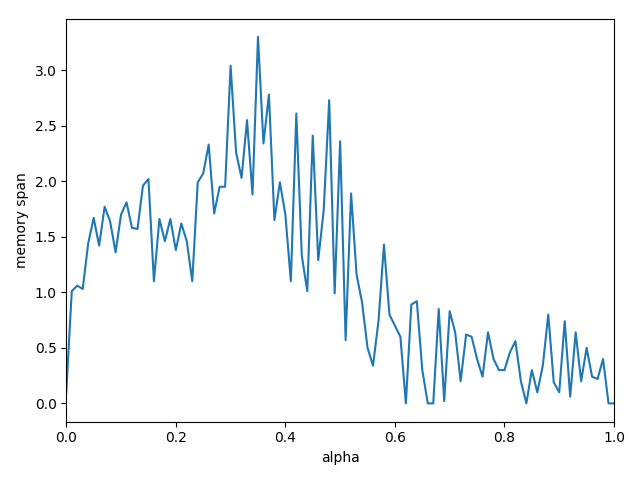
\includegraphics[width=\textwidth]{assets/r_memory_span}
        \caption{RecSOM hodnoty pamäťových hĺbok}
    \end{figure}
    
    \begin{figure}[H]
        \centering
        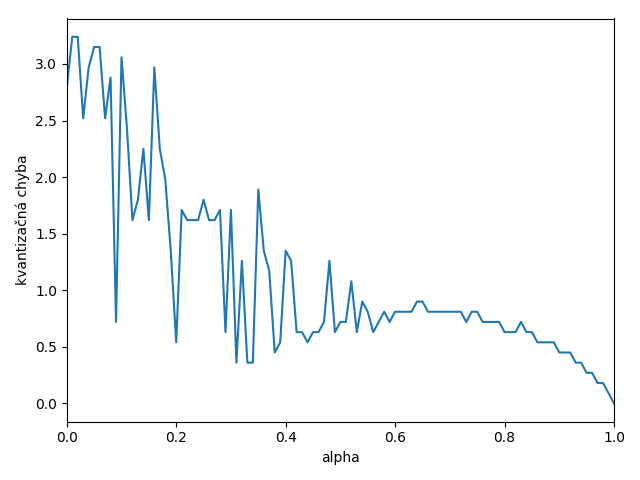
\includegraphics[width=\textwidth]{assets/r_errors}
        \caption{RecSOM hodnoty kvantizačných chýb}
    \end{figure}

\subsection{Analýza výsledkov RecSOM}
Keďže pri RecSOM máme iba jeden parameter, na vizualizáciu pamäťových hĺbok sme použili jednoduchý graf hodnôt.
Hodnoty na x-ovej osy sú hodnoty parametra $\alpha$  a na y-ovej osy sú hodnoty pamäťových hĺbok. 
Čísla v jednotlivých políčkach sú pamäťové hĺbky na konci poslednej epochy pre určitú hodnotu parametra $\alpha$.

RecSOM dosiahla najvyššie hodnoty pamäťovej hĺbky pri 
hodnotách parametra $\alpha = 0.76-0.82$, $\alpha = 0.85-0.87$ a $\alpha = 0.89,0.9,0.91,0.95$. 
Najnižšiu hodnotu dosiahla keď je $\alpha = 0$, čiže keď nepracuje so žiadnym kontextom, iba s aktuálnymi vstupmi.
Z grafu kvantizačných chýb vidíme, že sieť dosahuje minimálnu kvanizačnú chybu pri tých
hodnotách parametra $\alpha$, pri ktorých dosahuje aj najvyššiu pamäťovú hĺbku. 

Vyššia kvantizačná chyba je pri stredných hodnotách parametra $\alpha$, kde má aktuálny vstup aj kontext podobnú váhu a nedokáže sa na danom počte epôch správne natrénovať.
So zväčšovaním parametra $\alpha$, teda váhy kontextu, klesá aj kvantizačná chyba.
Najvyššia kvantizačná chyba je pri hodnotách najvyšších hodnotách parametra $\alpha$, je to z toho dôvodu, že sieť 
pracuje už iba s kontextom a aktuálny vstup má minimálny vplyv, preto sa nedokáže správne natrénovať, alebo potrebuje viacej trénovacích epôch.
Príčinou môže byť tiež rozdiel v dimenziách váhových vektorov a kontextových vektorov. Kontextové vektory majú v našom prípade omnoho vyššiu dimenziu (400) ako váhové vektory (26) a 
teda kontextová zložka vzdialenosti má prirodzene vyššie hodnoty, čo negatívne ovplyvňuje trénovanie siete pri vysokých hodnotách parametra $\alpha$.
Trénovanie RecSOM bolo relatívne pomalé v porovnaní s MSOM, najmä kvôli veľkosti kontextu a sieť dosiahla uspokojivé výsledky.

% todo ukazka priebehu klesacujec kvantizacnej chyby pri najvhodnejsej kombinacii parametrov
% todo priemer kvantizacnych chyb s hodnotou najlepsieho parametra
% ukazka testov s najlepsimi parametrami

% výsledky experimentu

\subsection{Activity RecSOM}
Keďže pri obyčajnej verzii RecSOM nevieme ovplyvniť žiadnym parametrom výpočet kontextu. Preto sme sa 
rozhodli vytvoriť si modifikovanú verziu RecSOM. Rozdiel oproti pôvodnej verzii je v spôsobe počítania 
aktivácie neurónov v kontexte. 
Upravili sme pôvodný vzorec % (pridat poznamku pod ciarov)
\begin{equation}
    y_{i} = \exp{(-d_{i})}
\end{equation}
tak aby obsahoval parameter $\beta$.
\begin{equation}
    y_{i} = \exp^{(-\beta \cdot d^2)}
\end{equation}

Hodnota $d^2$ je umocnená euklidovská vzdialenosť neurónu v mriežke od víťazného neurónu.
Na výpočet aktivity neurónu teda používame gaussovskú funkciu, ktorej "strmosť" ovplyvňujeme
pomocou $\beta$ parametra. To znamená, že ovplyvňujeme rozdiely medzi hodnotami aktivácie víťazného neurónu
a susedných neurónov. Táto funkcia je podobná funkcii susednosti, ktorá sa používa počas trénovania. 

Pre malé hodnoty parametra $\beta$ hodnoty aktivácie neurónov so stúpajúcou vzdialenosťou od víťaza
klesajú pomaly. 

Čím je $\beta$ parameter väčší tým je táto funkcia strmšia (väčší skok), čo znamená, že víťaz bude mať výrazne vyššiu hodnotu aktivácie
ako neuróny, ktorých vzdialenosť $d$ od vstupu a kontextu je vyššia.

\begin{figure}[H]
    \centering
    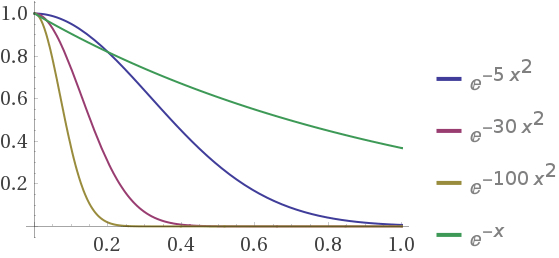
\includegraphics[width=\textwidth]{assets/plots}
    \caption{Grafy priebehu funkcií na výpočet aktivácií neurónov v Activity RecSOM}
\end{figure}
Na grafe je možno vidno rozdiely v priebehoch tejto funkcie s rôznymi hodnotami parametra $\beta$. Zelenou 
je vyznačený priebeh funkcie aktivácie, ktorý je používaný v pôvodnej RecSOM.

Samotnú hodnotu aktivácie sme chceli ešte normalizovať sumou všetkých aktivácii:
\begin{equation}
    y_{i} = \frac{\exp^{(-\beta \cdot d_{i}^{2})}}{\sum_{j} \exp^{(-\beta \cdot d_{j}^{2})}}
\end{equation}
Pri použití normalizácie sme dostávali signifikantne horšie výsledky
ako bez použitia normalizácie. Dôvodom bolo pravdepodobne to, že vychádzali veľmi malé
hodnoty aktivácií a rozdiely boli takmer veľmi malé. Z tohto dôvodu sme zostali 
pri pôvodnej nenormalizovanej verzii.

V prípade ak je hodnota aktivácie normovaná, potom môžeme túto
hodnotu interpretovať aj nasledovne:
Aktivita neurónu vyjadruje bayesovskú pravdepdobnosť, že vstup zodpovedá reprezentácii vo váhach daného neurónu.

\subsection{Activity RecSOM parametre}
V našom experimente sme vyskúšali kombinácie parametrov $\alpha$ a $\beta$.
Hodnoty parametra $\alpha$ sme zvolili z intervalu $<0, 1>$ s krokom $0.1$
Hodnoty parametra $\beta$ sme zvolili tak aby sme otestovali rôzne strmosti aktivačnej funkcie.
Konkrétne sme použili tieto hodnoty: $[5.0, 12.0, 13.0, 14.0, 15.0, 20.0, 30.0, 40.0, 50.0, 100.0]$
Pustili sme trénovanie na všetkých kombináciach parametrov $\alpha$ a $\beta$.

\subsection{Výsledky pre Activity RecSOM}

\begin{table}[h!]
    \centering
    \begin{tabular}{|c|c|} 
     \hline
     Parameter & Hodnota \\ 
     \hline\hline
     Hodnoty alpha & 0 - 1 (krok 0.1) \\ 
     \hline
     Hodnoty beta & [5.0, 12.0, 13.0, 14.0, 15.0, 20.0, 30.0, 40.0, 50.0, 100.0]\\ 
     \hline
     Veľkosť & 20x20  \\
     \hline
     počet epôch trénovania & 10  \\
     \hline
     veľkosť posuvného okna & 10  \\
     \hline
    \end{tabular}
    \caption{Parametre Activity RecSOM siete}
    \label{table:1}
    \end{table}
    
    \begin{figure}[H]
        \centering
        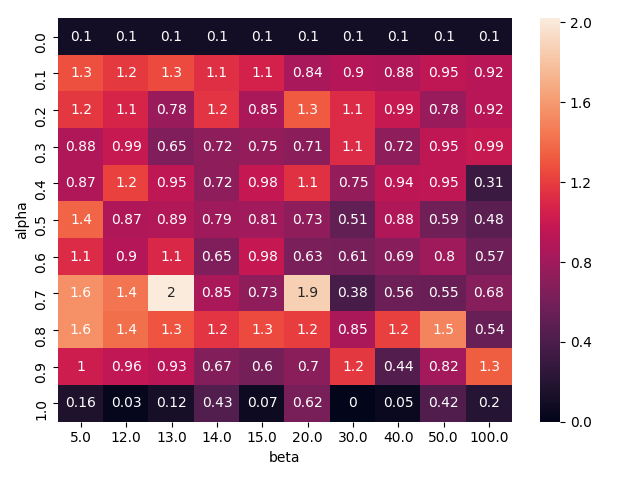
\includegraphics[width=\textwidth]{assets/ar_memory_span}
        \caption{Activity RecSOM hodnoty pamäťových hĺbok}
    \end{figure}
    
    \begin{figure}[H]
        \centering
        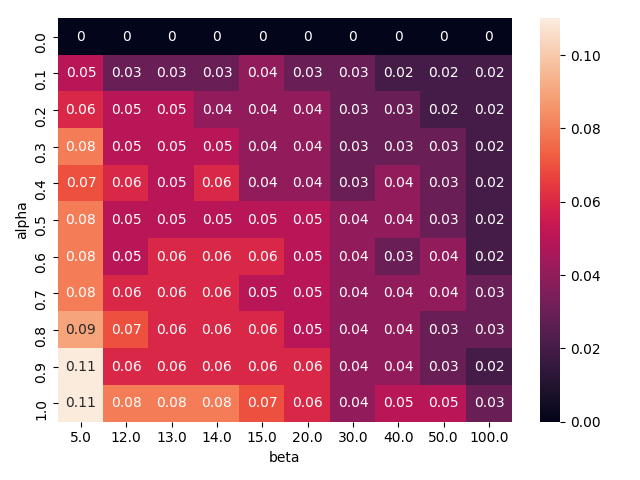
\includegraphics[width=\textwidth]{assets/ar_errors}
        \caption{Activity RecSOM hodnoty kvantizačných chýb}
    \end{figure}
    
\subsection{Analýza výsledkov Activity RecSOM}
Na x-ovej osy sú hodnoty parametra $\beta$ a na y-ovej osy sú hodnoty parametra $\alpha$.
Na grafe pamäťových hĺbok pre Activity RecSOM môžeme vidieť vysoké hodnoty pri hodnotách $\alpha = 1.0/0.9 a \beta = 5.0$.
Tieto však nie sú relevantné a sú spôsobené tým, že niektoré neuróny boli víťazmi iba jeden krát a dĺžka 
najdlhších spoločných podpostupností je pre ne rovná dĺžke posuvného okna. Je to možno vidieť na 
receptívnom poli siete pre parametre s hodnotami $\alpha = 1.0 a \beta = 5.0$ po poslednej trénovacej epoche:

\begin{lstlisting}
[["7""8""2""63""17"""""""""""""""""""""""""""""""]
["844""3""""""""6"""""""""""""""""""""""""""""]
["aacabddabd1"""""""""""""""""""""""""""""""""""""""]
["2""""""""11""""""""""""""acdabcbdba1"""""""""""""""""]
["""""""""""""""""""""""2"""""""""""""""""]
["""""6"""""""""""""""""""""""""""""""""""]
["10"""""""""""""""""""""""""""""""""""""""]
[""""""""""""""""""""""""""""""""""""""""]
[""""""""""""""""""""""""""""""""""""""""]
[""""""""""""""""""""""""""""""""""""""""]
["""""5"""""""""""""""""""""""""""""""""""]
[""""""""""""""""""""""""""""""""""""""""]
[""""""""""""""""""""""""""""""""""""""""]
[""""""""""""""""""""""""""""""""""""""""]
[""""""""""""""""""""""""""""""""""""""""]
["cadacdabcb1"""""""""""""""""""""""""""""""""""""""]
[""""""""""""""""""""""""""""""""""""""""]
["""""""""""""""""""""""""""""""cdbcadacda1"""""""""]
[""""""""""""""""""""""""""""""""""""""""]
[""""""""""""""""""""""""""""""""""""""""]]
\end{lstlisting}

Políčka s číslami označujú neuróny, ktorých pamäťové okno obsahuje uložené sekvencie, ale nemajú žiadnu 
spoločnú podpostupnosť.
Zvyšné políčka zobrazujú najdlhšiu spoločnú podpostupnosť spoločne s celkovým počtom podpostupností 
v danom pamäťovom okne neurónu. Na tomto receptívnom poli je vidno, prečo je hodnota pamäťovej hĺbky vysoká.

Najvyšie (neskreslené) hodnoty pamäťovej hĺbky sieť dosahuje pri hodnotách $\beta = 30,40$ a $\alpha = 0.6$, kde je aj relatívne nízka kvantizačná chyba.
Najnižšie hodnoty pamäťovej hĺbky sieť dosahuje ak je hodnota parametra $\alpha = 1$, čiže ak sieť pracuje iba s kontextom a tiež v prípade, keď je hodnota 
$\alpha = 0$, kedy sieť nepracuje s kontextom do minulosti a teda ani nemôže mať pamäťovú hĺbku.
Výsledky Activity RecSOM z hľadiska maximálnej hĺbky pamäte nám ukazujú, že hodnota patametra $\beta$ nemá veľký vplyv
na pamäťovú hĺbku siete.
Zaujímavý pri Activity RecSOM je graf kvantizačných chýb, kde môžeme vidieť ako nám parametre ovplyvňujú
schopnosť siete správne sa natrénovať. Ak je hodnota parametra $\beta$ nízka a podiel kontextu (hodnota parametra $\alpha$) vo 
výpočte vzdialenosti vysoká, tak má sieť vyššiu kvantizačnú chybu. Zvyšovanie hodnoty $\beta$ parametra znižuje kvantizačnú chybu siete.
Pri vyšších hodnotách parametra $\beta$ majú neuróny blízke víťazovi výrazne vyššiu hodnotu aktivácie vďaka strmšiemu priebehu funkcie na výpočet aktivácie. 
Inými slovami, informácie uložené v kontexte sú viac sústredené na aktivitu víťazného neurónu. 
Podobne ako pri RecSOM rozdiel medzi dimenziami váhových vektorov (26) a kontextových vektorov (400) je veľký a vzdialenosť medzi kontextom a kontextovým vektorom
je vo výpočte vzdialenosti je kvôli tomu vyššia. Vyššie hodnoty parametra $\beta$ spôsobujú, že aktivita väčšiny neurónov v sieti je blízka nule, čo znižuje aj hodnotu
vzdialenosti medzi kontextovými váhami a kontextom a teda klesá aj kvantizačná chyba.
Výsledkom experimentu s Activity RecSOM je, že $\beta$ parameter síce minimálne ovplyvňuje pamäťovú hĺbku siete, ale znižuje kvantizačnú chybu (teda schopnosť siete sa správne natrénovať). 
Čas trénovania bol podobný ako pri RecSOM.

% ukazka testov s najlepsimi parametrami

\subsection{MSOM parametre}
Pri MSOM máme okrem $\alpha$ parametra, používaného pri výpočte vzdialenosti, opäť aj $\beta$ parameter, ktorý určuje váhu
váhového vektora víťaza z predchádzajúceho kroku $w_{i^{*}}$ a váhu kontextu
z predchádzajúceho kroku $y_{i^{*}}$ pri výpočte kontextu. Je nazývaný aj ako "zmiešavací" parameter
a určuje váhu jednotlivých zložiek vlastností víťazného neurónu v kontexte.
V našom experimente skúšame všetky kombinácie $\alpha$ a $\beta$ parametrov.
Hodnoty pre oba parametre sú z uzavretého intervalu $<0, 1>$ s krokom $0.1$ (100 experimentov).
Pri experimentovaní s MSOM sa snažíme zistiť aký vplyv má odlišný kontext, ktorý obsahuje iba informáciu
o víťazovi z predchádzajúceho kroku, na pamäťovú hĺbku siete. MSOM má veľkú výhodu v signifikantne 
vyššej rýchlosti učenia, vďaka zredukovanej dimenzie kontextu.

\subsection{Výsledky pre MSOM}

\begin{table}[h!]
    \centering
    \begin{tabular}{|c|c|} 
     \hline
     Parameter & Hodnota \\ 
     \hline\hline
     Hodnoty alpha & 0 - 1 (krok 0.1)  \\ 
     \hline
     Hodnoty beta & 0 - 1  (krok 0.1) \\ 
     \hline
     Veľkost & 20x20  \\
     \hline
     Počet epôch & 10  \\
     \hline
     Veľkosť posuvného okna & 10  \\
     \hline
    \end{tabular}
    \caption{Parametre MSOM siete}
    \label{table:1}
    \end{table}
    
    \begin{figure}[H]
        \centering
        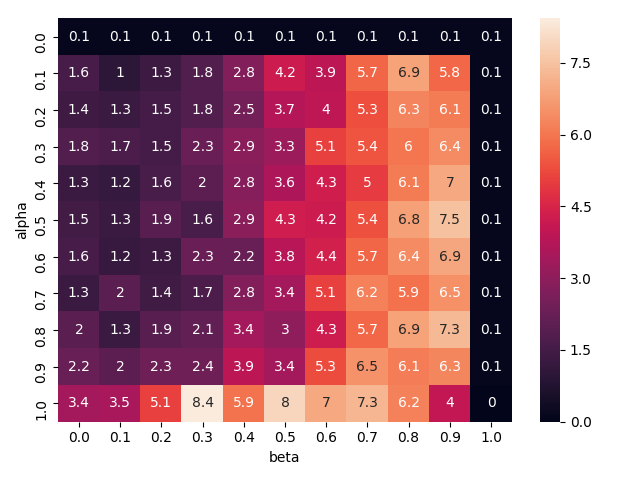
\includegraphics[width=\textwidth]{assets/m_memory_span}
        \caption{MSOM hodnoty pamäťových hĺbok}
    \end{figure}
    
    \begin{figure}[H]
        \centering
        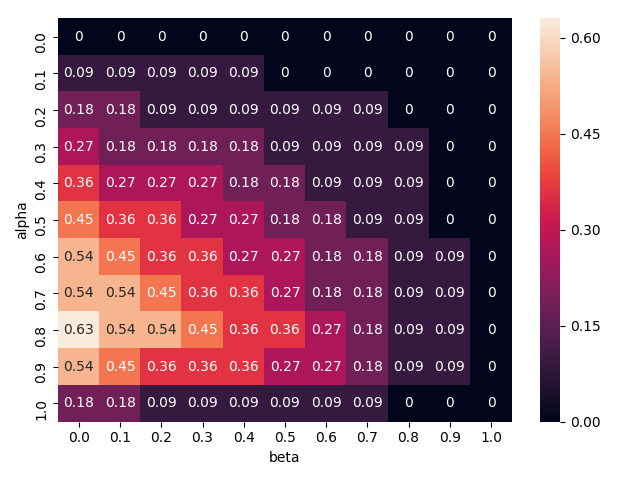
\includegraphics[width=\textwidth]{assets/m_errors}
        \caption{MSOM hodnoty kvantizačných chýb}
    \end{figure}

 Na x-ovej osy sú hodnoty parametra $\beta$ a na y-ovej osy sú hodnoty parametra $\alpha$. 
 Pamäťová hĺbka pri MSOM dosahuje minimá ak je jeden z parametrov $\alpha$ alebo $\beta$ nulový a teda sieť nemá
 žiadny alebo len minimálny kontext. Ak je $\alpha = 0$, tak sa zanedbáva kontextová zložka pri výpočte vzdialenosti a 
 teda aj pri samotnom trénovaní siete a keď je $\beta = 0$ tak sa zanedbávajú váhy víťaza z predchádzajúceho kroku pri výpočte kontextu.
 Minimum pamäťovej hĺbky MSOM dosahuje ak sú $\alpha$ aj $\beta$ nulové.

 MSOM dosahuje v priemere vysoké hodnoty pamäťovej hĺbky, pričom je to zároveň 
 výpočtovo najefektívnejšia verzia rekurentnej SOM pri nízko dimenzionálnych vstupoch. Ukazuje sa, že kontext redukovaný na vlastnosti víťaza z predchádzajúceho kroku
 neovplyvňuje negatívne pamäťvú hĺbku siete.
 Maximálne (neskreslené) hodnoty pamäťovej hĺbky dosahuje pri nízkych hodnotách $\alpha = 0.1-0.4$, čo znamená že pri výpočte vzdialenosti má vyššiu váhu vzdialenosť vstupu od 
 váhového vektora ako vzdialenosť kontextu od kontextového vektora (Pri MSOM sú hodnoty vzdialeností porovnateľné, keďže kontext a vstup majú rovnaké dimenzie). 
 Pri maximách je hodnota parametra $\beta$ sú $1.0$, čo znamená, že pre pamäťovú hĺbku MSOM je dôležité zloženie kontextu z predchádzajúceho kroku.
 Najvyššie hodnoty kvantizačnej chyby sieť dosahuje keď je $\alpha = 0.8$ a $\beta = 1.0$.



% vyhodnotenie vysledkov experimentu

% ukazka testov s najlepsimi parametrami

\subsection{Decaying MSOM}
Pre potreby nášho experimentu sme si vytvorili ďalšiu modifikovanú verziu % prida poznamku pod ciarou
rekurentnej SOM. Pri RecSOM kontext tvorí vektor aktivácii všetkých neurónov z predchádzajúceho kroku, 
pri MSOM je to kombinácia vlastností víťazného neurónu z predchádzajúceho kroku. 
Preto sme sa rozhodli použiť odlišný typ kontextu, ktorý bude tvorený kombináciou predchádzajúcich vstupov 
siete a nie stavmi siete z minulých krokov. To znamená, že kontext nie je ovplyvnený samotným procesom trénovania
ani tým, čo sa sieť naučila v predchádzajúcich krokoch, ale iba samotnými vstupnými dátami.
Zvyšné vlastnosti siete zostávajú rovnaké ako v iných rekurentných SOM.

Kontext počítame pomocou nasledujúceho rekurzívneho vzťahu:
\begin{equation}
    c_{t} = x_{t} + \beta * c_{t-1}
\end{equation}
ktorý v rozvinutej forme môžeme zapísať ako:
\begin{equation}
	c = \beta^{0} \cdot x_{t} + \beta^{1} \cdot x_{t-1} + 
	\beta^{2} \cdot x_{t-2} \ddots \beta^{n} \cdot x_{t-n}
\end{equation}

$\beta$ parameter je číslo z intervalu $\beta < 1 \wedge \beta > 0$ a
$x_t, x_{t-1}, x_{t-2} ...$ sú vstupné vektory z predchádzajúcich krokov.
$t$ je číslo aktuálneho kroku a $n$ je veľkosť trénovacej množiny.

Z rekurzívneho vzťahu vyplýva, že kontext je tvorený kombináciou predchádzajúcich vstupov,
pričom čím dávnejší je vstup, tým menšiu váhu má vo výslednom kontexte, čo je zabezpečené umocňovaním
$\beta$ parametra. Toto sa nazýva leaky integration. V našom prípade
to znamená, že dávne vstupy postupne strácajú na dôležitosti, pričom sa stále sa podieľajú 
na vytváraní výsledného kontextu.

Čím je hodnota parametra $\beta$ vyššia, tým viac informácii z predchádzajúcich vstupov v sebe
kontext obsahuje. Dôležitosť dávnejších vstupov exponenciálne klesá.

\subsection{Decaying MSOM parametre}
V experimente opäť skúšame všetky kombinácie $\alpha$ a $\beta$ parametrov.
Hodnoty pre oba parametre sú z uzavretého intervalu $<0, 1>$ s krokom $0.1$.

\subsection{Výsledky pre Decaying MSOM}
\begin{table}[h!]
    \centering
    \begin{tabular}{|c|c|} 
     \hline
     Parameter & Hodnota \\ 
     \hline\hline
     Hodnoty alpha & 0 - 1 (krok 0.1)  \\ 
     \hline
     Hodnoty beta & 0 - 1  (krok 0.1) \\ 
     \hline
     Veľkosť & 20x20  \\
     \hline
     Počet epôch trénovania & 10  \\
     \hline
     Veľkosť posuvného okna & 15 \\
     \hline
    \end{tabular}
    \caption{Parametre Decaying MSOM siete}
    \label{table:1}
    \end{table}
    
    
    \begin{figure}[H]
        \centering
        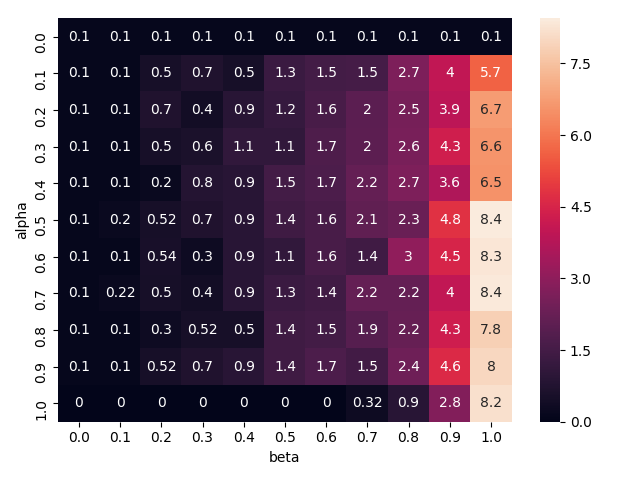
\includegraphics[width=\textwidth]{assets/dm_memory_span}
        \caption{Decaying MSOM hodnoty pamäťových hĺbok}
    \end{figure}
    
    \begin{figure}[H]
        \centering
        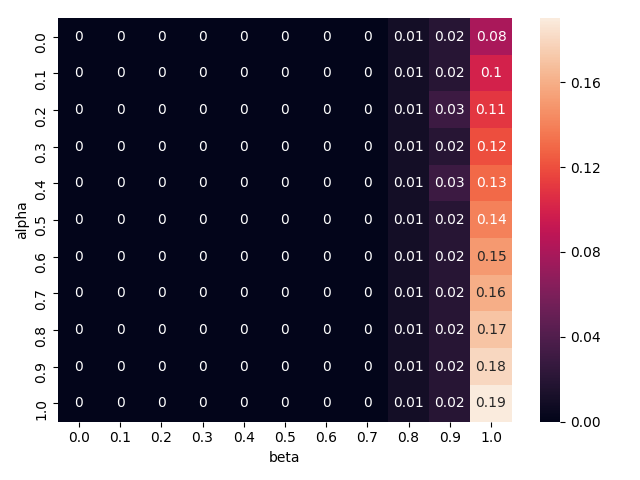
\includegraphics[width=\textwidth]{assets/dm_errors}
        \caption{Decaying MSOM hodnoty kvantizačných chýb}
    \end{figure}

    
Na x-ovej osy sú hodnoty parametra $\beta$ a na y-ovej osy sú hodnoty parametra $\alpha$.
Decaying MSOM dosahuje veľmi vysoké hodnoty pamäťových hĺbok. 
V receptívnom poli je však vidno, že je to pamäťovými oknami, ktoré obsahujú iba jednu sekvenciu. Čo trochu skresľuje výsledky.
Na grafe kvantizačných chýb je možno vidieť, že sieť sa učí veľmi dobre v prípade, že je $\beta < 1$. Ak je $\beta = 1$ kvantizačná chyba stúpa, keďže všetky minulé vstupy siete
majú rovnakú váhu, sieť sa nie je schopná správne natrénovať.
Týmto experimentom sme vyskúšali aký vplyv na pamäťovú hĺbku siete má úplne odlišný druh kontextu a či sme s ním schopný sieť natrénovať.
Ukázalo sa, že s takýmto kontextom dokážeme dosiahnuť podobné výsledky ako s RecSOM. 
Pri predchádzajúcich rekurentných sieťach kontext obsahuje reprezentáciu vplyvov jednotlivých minulých vstupov na sieť a tu je to kombinácia samotných minulých vstupov siete. 
% vyhodnotenie vysledkov experimentu

% ukazka testov s najlepsimi parametrami

\section {Porovnanie výsledkov SOM}
Po nájdení ideálnych parametrov pre všetky 3 typy sietí, sme spustili 5 behov pre tieto kombinácie parametrov a všetky 3 trénovacie množiny,
pričom sme použili rovnakú počiatočnú inicializáciu váh a spravili priemer týchto hodnôt. Zvyšné hodnoty parametrov sme ponechali
rovnaké ako pri hľadaní optimálnych parametrov.

Výsledky pre hodnoty parametra $\alpha = $ a $\beta = $
\subsection{RecSOM}
\begin{itemize}
    \item \textbf{abcd}
    \item \textbf{reber}
    \item \textbf{corpus}
\end{itemize}

\begin{figure}[H]
    \centering
    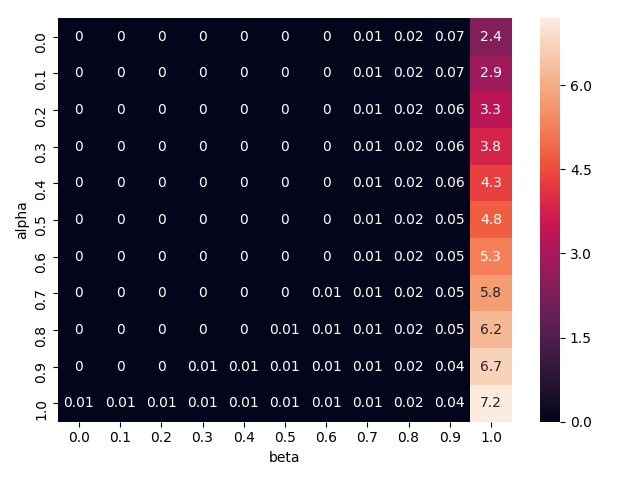
\includegraphics[width=\textwidth]{assets/decay_msom_errors}
    \caption{Graf klesajúcej kvantizačnej chyby počas trénovania}
\end{figure}



\subsection{Activity RecSOM}
Výsledky pre hodnoty parametra $\alpha = $ a $\beta = $
\begin{itemize}
    \item \textbf{abcd}
    \item \textbf{reber}
    \item \textbf{corpus}
\end{itemize}

\begin{figure}[H]
    \centering
    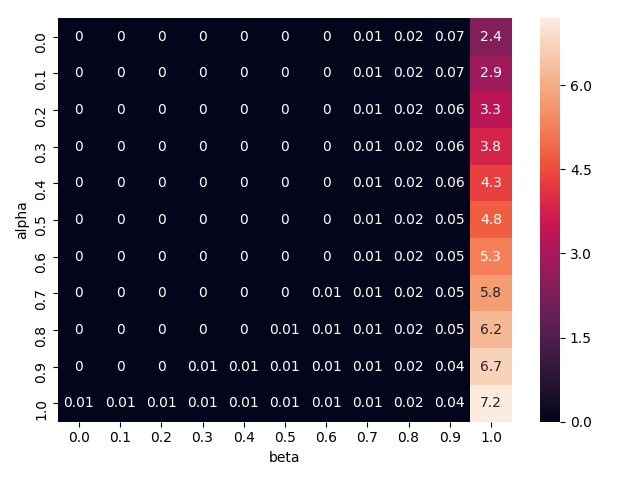
\includegraphics[width=\textwidth]{assets/decay_msom_errors}
    \caption{Graf klesajúcej kvantizačnej chyby počas trénovania}
\end{figure}



\subsection{MSOM}
Výsledky pre hodnoty parametra $\alpha = $ a $\beta = $
\begin{itemize}
    \item \textbf{abcd}
    \item \textbf{reber}
    \item \textbf{corpus}
\end{itemize}

\begin{figure}[H]
    \centering
    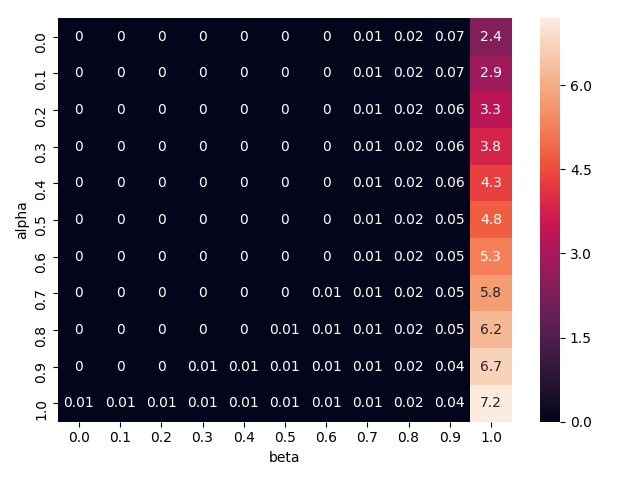
\includegraphics[width=\textwidth]{assets/decay_msom_errors}
    \caption{Graf klesajúcej kvantizačnej chyby počas trénovania abcd}
\end{figure}



\subsection{Decay MSOM}
Výsledky pre hodnoty parametra $\alpha = $ a $\beta = $
\begin{itemize}
    \item \textbf{abcd}
    \item \textbf{reber}
    \item \textbf{corpus}
\end{itemize}

\begin{figure}[H]
    \centering
    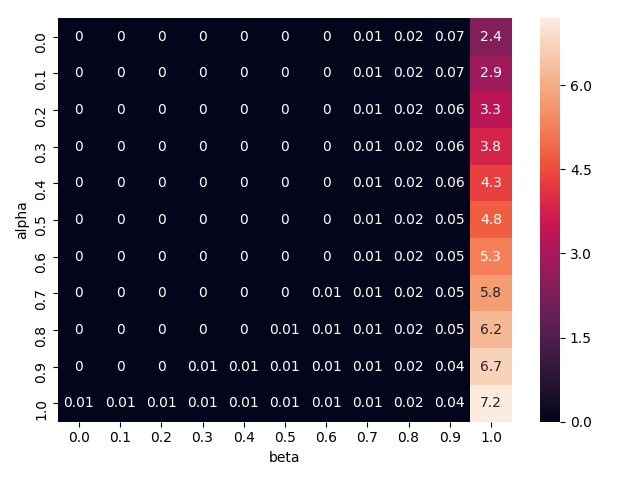
\includegraphics[width=\textwidth]{assets/decay_msom_errors}
    \caption{Graf klesajúcej kvantizačnej chyby počas trénovania abcd}
\end{figure}



\section{ Vyhodnotenie experimentu }
Experimentami sme zistili, že na hĺbku pamäte je najviac ovplyvnená zložením samotného kontextu rekurentnej SOM.
Parametre, ktoré sme testovali a ktoré vplývajú na hĺbku pamäte rekurentných SOM sú $\alpha$ a $\beta$
$\alpha$ vystupuje vo vzťahu pre výpočet vzdialenosti vstupu od určitého neurónu v sieti.
$\beta$ zase ovplyvňuje výpočet samotného kontextu.
Pre nízkodimenzionálne vstupy je najvhodnejšie použiť MSOM, ktorá je výpočtovo najefektívnejšia a dosahuje veľmi dobré 
výsledky.
Pre vysokodimenzionálne vstupy je z hľadiska veľkosti kontextu a výpočtovej náročnosti vhodnejšie použiť RecSOM alebo
Activity RecSOM.


\section{Experiment so SRN a Reberovým automatom}
SRN má niektoré vlastnosti podobné s RecSOM.
V RecSOM máme vrstvu neurónov, ktorá je prepojená s kontextovou vrstvou, podobne 
aj v SRN s Elmanovou architektúrou máme skrytú vrstvu, ktorá je prepojená s kontextovou vrstvou.
Túto analógiu je dobre vidieť ak by sme z Elmanovej siete odstránili výstupnú vrstvu a ponechali iba 
vstupnú, skrytú a kontextovú vrstvu, potom nám zostane architektúra RecSOM siete.
Spôsob trénovania a rozmiestňovania vstupov v priestore je úplne odlišný v prípade Elmanovej siete.

Naším hlavným cieľom pri tomto experimente s SRN bolo preskúmať vlastnosti siete a pokúsiť sa nájsť 
spôsob merania a vyhodnotenia jej pamäťovej hĺbky. 
Tiež sme chceli preskúmať niekoľko zaujímavých vlastností SRN.

Prvá časť experimentu s SRN prebiehala v nasledujúcich krokoch:
\begin{itemize}
    \item Podobne ako pri experimentoch so samoorganizujúcimi sa mapami, ako prvé sme si potrebovali vytvoriť vhodnú trénovaciu množinu.
     Rozhodli sme sa, že použijeme podobné zloženie trénovacej množiny ako pri samoorganizujúcich sa mapách.
     Vstupom je vždy jedno písmeno z náhodne generovanej sekvencie písmen $abcd$ a ako očakávaný výstup je vždy nasledujúce písmeno v sekvencii.
     Takýmto spôsobom sme vytvorili mnnožinu trénovacích príkladov.
     \item Zvolili sme si vhodné aktivačné funkcie:  \\
     Ako aktivačnú funkciu na skrytej vrstve sme použili hyperbolický tangens.
     \begin{equation}
         tanh(x) = \frac{e^{2x} - 1}{e^{2x} + 1}
     \end{equation}
     Aktivačnú funkciu na výstupnej vrstve sme použili softmax. 
     \item Následne sme museli overiť funkčnosť našej implementácie siete. Ako chybovú funkciu sme použili log loss.
    Počas testovania nám chyba klesala a sieť po natrénovaní predikovala korektné výsledky na testovacích sekvenciách.
     \item Keď sme mali funkčnú implementáciu SRN Elmanovej siete, natrénovali sme ju na našej trénovacej množine.
     Parametre, ktoré sme použili počas trénovania: \\
    \begin{table}[h!]
        \centering
        \begin{tabular}{|c|c|} 
        \hline
        Parameter & Hodnota \\ 
        \hline
        veľkosť skrytej vrstvy & 30  \\
        \hline
        počet epôch & 100  \\
        \hline
        veľkosť posuvného okna na trénovacej množine & 3  \\
        \hline
        počet krokov do minulosti (T) & 5 \\
        \hline
        \end{tabular}
        \caption{Parametre SRN s Elmanovou architektúrou}
        \label{table:1}
    \end{table}
\end{itemize}

SRN si na skrytej vrstve vytvára určitú reprezentáciu vstupov. Preto sme sa rozhodli, že 
správne natrénovanej SRN budeme postupne predkladať písmená z trénovacej množiny, pričom si po každej predikcii, ktorú sieť spraví,
 uložíme aktivácie neurónov (vektor) na skrytej vrstve siete do nejakej množiny. 
Ku každému takémuto vektoru priradíme posuvné okno daného znaku z trénovacej množiny (podobne ako pri experimentoch so SOMkami). 
Po predložení všetkých znakov z trénovacej množiny sieti sme dostali dvojice posuvných okien s prislúchajúcimi aktiváciami neurónov
na skrytej vrstve siete. \\

Tieto dáta sme potrebovali nejakým spôsobom vizualizovať, aby sme v nich vedeli identifikovať prípadné súvislosti medzi reprezentáciou vstupov na skrytej vrstve a 
podobnosťou samotných vstupov.
Rozhodli sme sa, že použijeme vizualizáciu pomocou dendrogramu.
Vizualizácie vo forme dendrogramu sa často používajú ak potrebujeme vizualizovať hierarchické klastrovanie dát.

Na vytvorenie denrogramu potrebujeme vytvoriť tzv. podobnostnú maticu (ang. similarity matrix), kde 
riadky aj stĺpce reprezentujú jednotlivé kontextové vektory a hodnoty v samotnej matici sú euklidovské vzdialenosti medzi týmito vektormi.
Z toho vyplýva, že na diagonále sú samé nulové hodnoty (rovnaké vektory majú medzi sebou nulovú vzdialenosť).

Z takejto matice potom vieme vytvoriť stromový graf, dendrogram, ktorý vizualizuje súvislosti medzi euklidovskou vzdialenosťou jednotlivých vektorov a samotnými posuvnými oknami z trénovacej množiny.
Z toho vieme potom povedať, ktoré postupnosti vstupov sú vo vnútornej reprezentácii SRN blízke. 

Takáto reprezentácia nám hovorí o tom, ako sieť interne reprezentuje dáta z trénovacej množiny.

\begin{figure}[H]
    \centering
    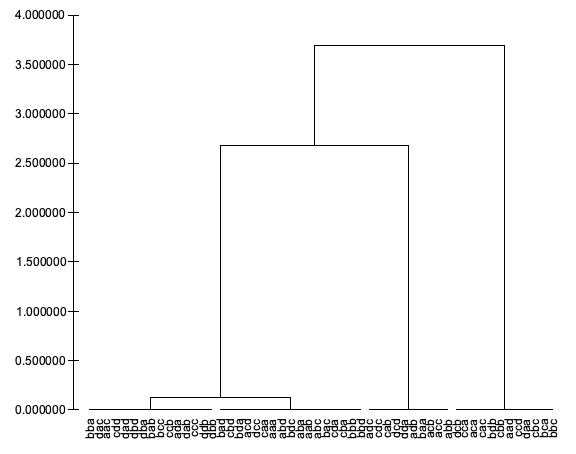
\includegraphics[width=\textwidth]{assets/dendrogram}
    \caption{Dendrogram pre Elmanovu sieť. Na x-ovej osy sú posuvné okná a na y-ovej osy sú vzdialenosti medzi jednotlivými vektormi}
\end{figure}

Na dendrograme vidíme, že pre sieť podobné vstupy majú rovnakú euklidovskú vzdialenosť vektorov.
V našej sieti sa vytvorili 4 klustre podobnej veľkosti. Nehovorí nám to bohužiaľ nič o pamäťovej hĺbke Elmanovej siete.
Nevieme ju z takejto vizualizcáie kvantifikovať.

\subsection{Stavový automat na skrytej vrstve}
Zaujímavou vlastnosťou SRN je aj to, že si na skrytej vrstve dokáže vytvoriť vlastnú reprezentáciu stavového automatu, ak 
je trénovaná na trénovacej množine, ktorá je tvorená reťazcom generovaným napríklad reberovým automatom \cite{Servan-Schreiber1991}
Vďaka tejto vlastnosti by sa mala SRN natrénovať na takejto trénovacej množine s nulovou chybou.
Túto vlastnosť sme sa rozhodli overiť.
Vytvorili sme si podobnú trénovaciu množinu ako pri prvom experimente.
Parametre, ktoré sme použili na natrénovanie siete na takejto množine dát:
\begin{table}[h!]
    \centering
    \begin{tabular}{|c|c|} 
    \hline
    Parameter & Hodnota \\ 
    \hline
    veľkosť skrytej vrstvy & 30  \\
    \hline
    počet epôch & 100  \\
    \hline
    počet krokov do minulosti (T) & 5 \\
    \end{tabular}
    \caption{Parametre SRN s Elmanovou architektúrou - reberové reťazce}
    \label{table:1}
\end{table}
Výsledkom tohto trénovania je potvrdenie skutočnosti, že sieť sa dokázala 
natrénovať po 100 epochách s nulovou trénovacou chybou na reťazcoch generovaných reberovým automatom, 
čiže si na svojej skrytej vrstve dokázala vytvoriť reprezentáciu stavového automatu.






